\documentclass[12pt]{article}
\usepackage{amsmath}
\usepackage{graphicx}
\usepackage{siunitx}
\usepackage{wrapfig}
\usepackage{multicol}
\usepackage{xcolor}
\usepackage[utf8]{inputenc}



\begin{document}


\title{Controllable Variable Intensity LED Light  \\ Lab Report 3 \\ ELP100}
\author{Deevyansh Khadria\\ 2022EE31883 \\ Group 27}
\maketitle

\vspace{15px}
\tableofcontents






\newpage
\section{Aim}
    To design a circuit for controllable and variable intensity of LED light 
\section{Apparatus}
    \begin{enumerate}
        \item BC547 transistor 
        \item LED 
        \item Power Supply 
        \item Resistors     
    \end{enumerate}
\section{Theory}
    \begin{enumerate}
        \item The dimming and intensity control of an LED using a BC547 transistor is a  common electronic circuit design. The BC547 is a NPN bipolar junction  transistor (BJT) that is commonly used in electronic circuits as a switch or  amplifier. In this circuit, the BC547 is used to control the current flowing  through an LED, thereby controlling its brightness. 
        \item The circuit works by adjusting the base voltage of the BC547 transistor.  The base voltage is controlled by a potentiometer, which is wired to the  
        base of the transistor. The potentiometer allows for the adjustment of the  base voltage, which in turn controls the current flowing through the LED.  As the base voltage increases, the current flowing through the LED also  increases, causing the LED to become brighter. Conversely, as the base  voltage decreases, the current flowing through the LED decreases, causing  the LED to become dimmer. 
        \item Additionally, a 10K resistor is included in the circuit to protect the transistor  from damage. The resistor limits the current flowing through the base of  the transistor, preventing excessive current from damaging the transistor.
        \item In summary, this circuit uses a BC547 transistor to control the current  flowing through an LED, which in turn controls the LED's brightness. The  circuit works by adjusting the base voltage of the transistor through a  potentiometer, and the circuit is protected by a 10K resistor that limits the  current flowing through the base of the transistor.
    \end{enumerate}

    
    \begin{figure}[h!]
        \centering
        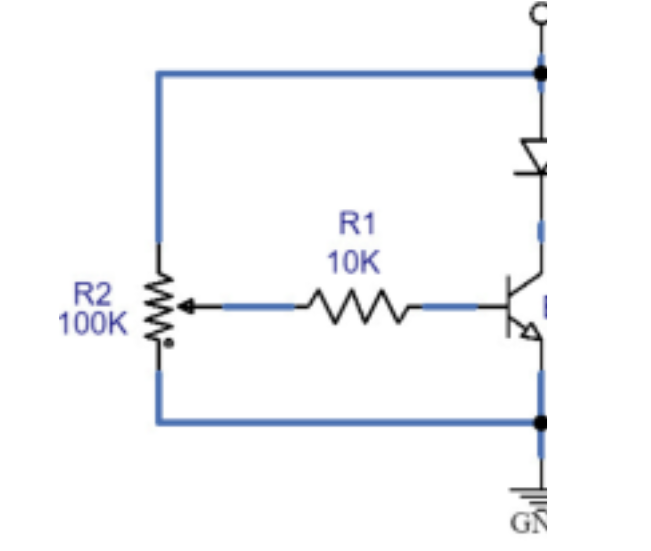
\includegraphics[width=0.5\linewidth]{setup.png}
        \caption{Caption}
        \label{fig:enter-label}
    \end{figure}
    \begin{multicols}{2}
    \begin{center}
        
   
    \fcolorbox{black}{white}{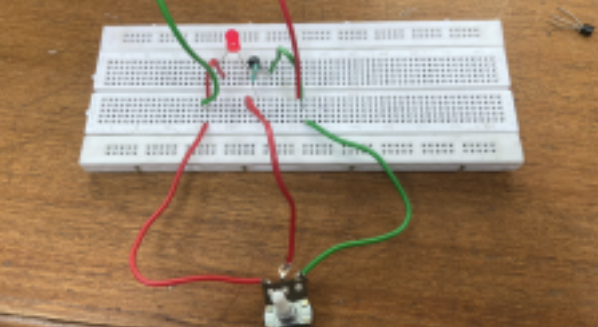
\includegraphics[width=0.9\linewidth]{Breadboard.png}}
    \columnbreak
    \fcolorbox{black}{white}{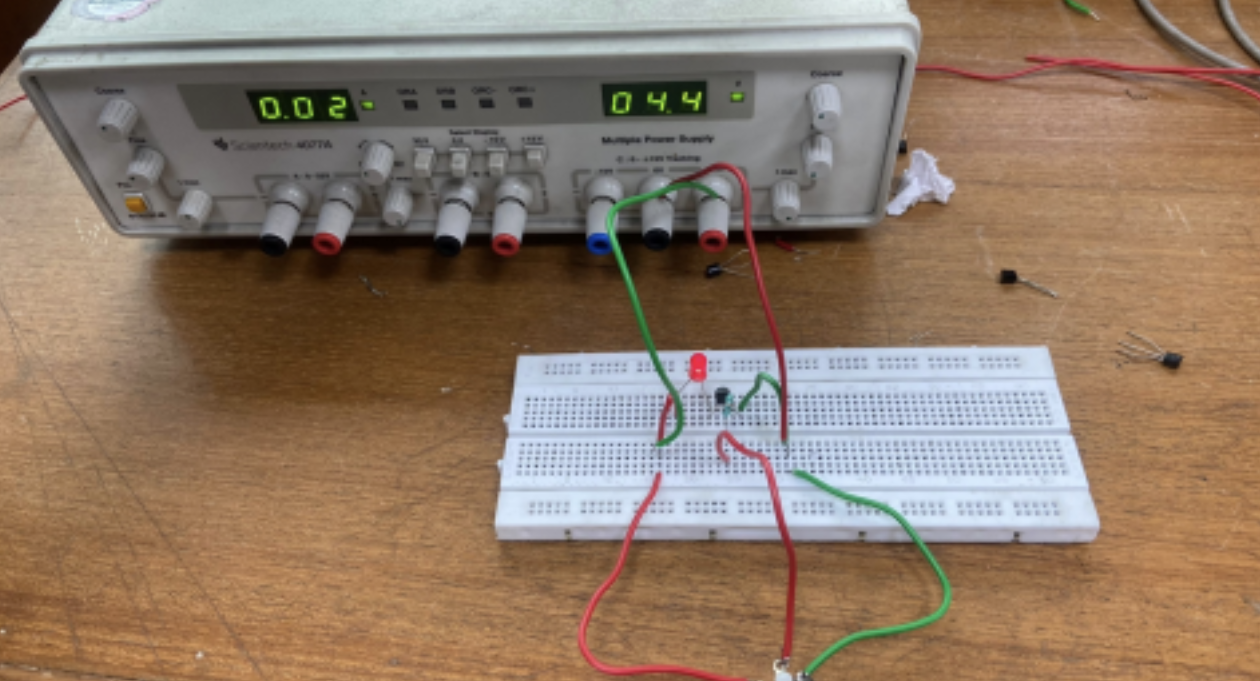
\includegraphics[width=0.9\linewidth]{Result.png}}
    \end{center}
    \end{multicols}
    
    
    
    
    

    
\section{Conclusions}
    \begin{enumerate}
        \item The conclusion of the dimming and intensity control of an LED using a  BC547 transistor experiment is that a simple circuit can be designed to  control the brightness of an LED by adjusting the base voltage of a BC547  transistor.  
        \item The circuit works by connecting a potentiometer to the base of the  transistor, which allows for the adjustment of the base voltage. As the base  voltage increases, the current flowing through the LED also increases,  causing the LED to become brighter.  
        \item Conversely, as the base voltage decreases, the current flowing through the  LED decreases, causing the LED to become dimmer. 
        \item Additionally, a 10K resistor is included in the circuit to protect the transistor  from damage.
        \item In conclusion, the experiment demonstrates how a simple circuit can be  used to control the brightness of an LED and how the circuit components  interact to achieve this functionality. The experiment also highlights the  importance of proper circuit design, circuit protection and precautions that  should be taken while working with electronics.
    \end{enumerate}
\section{Source of Error}
    \begin{enumerate}
        \item Incorrect wiring: Incorrectly wiring the circuit can lead to errors in the  circuit's operation and can cause damage to the components.
        \item Incorrect component values: Using the wrong values for components  such as resistors or capacitors can cause errors in the circuit's  operation. 
        \item Power supply voltage variations: The voltage supplied by the power  supply may not be exactly the same as the voltage required by the  circuit, which can cause errors in the circuit's operation.
        \item Dirty or corroded components: Over time, components may become  dirty or corroded, which can cause errors in the circuit's operation.
        \item Temperature effects: Temperature changes can affect the performance  of electronic components, leading to errors in the circuit's operation.
        \item Human error: Misreading of the circuit diagram, incorrect component  placement, or any other human error may lead to circuit malfunction. 
    \end{enumerate}
\section{Precautions}
    \begin{enumerate}
        \item Always work with low voltage and current: Make sure to use a low  voltage power supply (9V) and low current (20mA) to avoid any electrical  hazards. 
        \item Handle components carefully: Transistors, LEDs, and other electronic  components are delicate and can be easily damaged. Handle them with  care and avoid dropping or applying excessive force to them. 
        \item Use the correct wiring diagram: Make sure to use the correct wiring  diagram for your circuit to avoid any errors or mistakes.
        \item Avoid short-circuits: Short-circuits can cause damage to the circuit and  even lead to a fire. Be careful not to touch any of the circuit components  while they are connected to the power supply
        \item Use proper protective equipment: Always wear safety goggles and  gloves while working with electronics. 
    \end{enumerate}
\end{document}

